Thermodynamics, generally speaking, is the science of energy. It focuses on the transformation of energy from one form to another.  This includes transforming heat into work, such as in an automobile engine or at a power plant, and transforming work into heat transfer, such as in refrigerators or heat pumps.

The application of Thermodynamics is almost everywhere in our daily life. Examples of some application areas of this subject are: propulsion, internal combustion engines, power plants, refrigeration and air conditioning, solar heating, the interaction of the human body with its surroundings, biomedical devices, the biology of the human body, animals, plants, ecological systems, etc. In this course on thermodynamics we will focus on the analysis of energy systems and the application of these systems to real world contexts.

There are two approaches of teaching Thermodynamics – microscopic and macroscopic. Classical thermodynamics (the macroscopic approach) does not require detailed knowledge of molecular motion to describe a system. Statistical Thermodynamics (the microscopic approach) considers quantum mechanical description of molecules. We will primarily be looking at the macroscopic view, while occasionally using the microscopic approach to improve our basic understanding.

This first chapter is dedicated to introductory concepts, dimensions, and units.
The basic principles of thermodynamics are the conservation of mass, the conservation of energy, and the concept of entropy.  Basic thermodynamics terminology covered in this chapter includes the concepts of a system, properties, states, equilibrium, and processes. 

We will distinguish primary dimensions in Thermodynamics such as mass ($m$), length ($L$), time ($t$), temperature ($T$), electric current ($I$), the amount of a substance ($n$), and secondary (or derived) dimensions such as: velocity ($\frac{\rm m}{\rm s}$), density ($\frac{\rm kg}{\rm m^3}$), pressure ($\frac{\rm N}{\rm m^2}$), etc. In this course we will use the two most prevalent unit systems: the International System of Units (SI) and the United States Customary Units (US), focusing primarily on the first.

%--------------------------------------------------------------------
\section{Thermodynamics and Energy}
%--------------------------------------------------------------------

Thermodynamics is the science of energy, including energy storage and energy in transit. The Conservation of Energy Principle states that energy cannot be created or destroyed, but can only change its form. The three forms of energy storage of greatest interest to us are Potential Energy ({\bf PE}), Kinetic Energy ({\bf KE}), and Internal Energy ({\bf U}), which we introduce below. The two forms of energy in transit that we consider are Work ({\bf W}) and Heat ({\bf Q}), and the interactions between these various forms of energy are defined in terms of the First Law of Thermodynamics.

%--------------------------------------------------------------------
\section{Force and Work}
%--------------------------------------------------------------------
\subsection{Nomenclature}
\begin{center}
\begin{tabular}{cccc}
  Symbol & Meaning & SI Units & English Units \\ \hline 
  $F$ & Force & Newton [N] & pounds-force [lbf] \\
  $m$ & Mass & kilogram [kg] & slugs OR pounds-mass [lbm] \\
  $a$ & Acceleration & $\text{meters}/\text{second}^2$ $[\accSI]$ & $\text{feet}/\text{second}^2$ $[\accE]$ \\
  $W$ & Work & Joules [J] & foot-pounds [ft-lb]
\end{tabular}\\
\end{center}
\subsection{Newton's Second Law}
You should have already seen Newton's Second Law in Engineering Physics.\\

Newton’s Second Law states:
\begin{equation*}
  F = m a
\end{equation*}

Mass ($m$) and force ($F$) are two of the most common dimensions we will be using in this course.  Mass is used in nearly everything, because we are typically using properties of matter given {\bf per unit mass}.  Force is used almost as often, but it tends to be hidden as energy ($F \cdot d = W [{\rm J}]$) or pressure ($F/ A = p\ [{\rm Pa}]$)
%($F [{\rm N}] \cdot d [{\rm m}] = W [{\rm J}]$) or pressure ($F\ [{\rm N}] / A\ [{\rm m^2}] = p\ [{\rm Pa}]$).

You'll notice above that there are two possible units for mass in the US system.  The US unit of slugs is not used from day-to-day, but it is the most direct analog of the SI unit kilograms [kg].  More commonly used is the pound-mass [lbm], which is defined by the amount of mass which creates a pound-force in Earth's standard gravity.\\

Since the acceleration due to gravity g = 32.2$\accE$ we have:
\begin{align*}
  1\:\text{lbf}\:&=32.2\:\accE \cdot 1\:\text{lbm} \\
  1\:\text{lbf}\:&=1\:\accE \cdot 1\:\text{slug} \\
  1\:\text{slug}\:&=32.2\:\text{lbm}
\end{align*}

%Unity Conservation Ratio:

%  \[\frac{N\times s^2}{kg\times m}=1\,\,\,\,\,\text{and}\,\,\,\,\,\frac{lbf\times s^2}{32.174,lbm\times ft}=1\]

\subsection{Work}

We now consider the work done ($W$), which is the energy transferred to an object in motion requiring both an applied force ($F$) and distance moved ($d$). If the force is constant over the distance moved then the work done is given by:
\begin{equation*}
  W=F d,
\end{equation*}

In general, however, the force is not constant over the distance. For varying forces we need to sum all the incremental work processes taking into consideration the variation of the force. This leads to the integral form for determining work done as follows:
\begin{equation*}
  W=\int_0^d F\,dx
\end{equation*}

Notice that the integral form can be simplified to the original form when $F$ is constant.

%--------------------------------------------------------------------
\section{Unit Conversions}
%--------------------------------------------------------------------

It is often necessary to convert data from one unit system to another.  The lists below give conversions for the basic units, along with several shortcuts for commonly used unit combinations.

\begin{multicols}{2}
\subsubsection{Base Units}
\begin{align*}
1 \text{ kg} & = 2.2 \text{ lbm} = 0.0685 \text{ slug} \\
1 \text{ lbm} & = 0.031 \text{ slug} = 0.4536 \text{ kg} \\
1 \text{ N} & = 0.225 \text{ lbf} \\
1 \text{ lbf} &= 4.448 \text{ N} 
\end{align*}

\begin{align*}
1 \text{ m} & = 3.281 \text{ ft} \\
1 \text{ ft} &= 0.3048 \text{ m} \\
1 \text{ cm} &= 0.3937 \text{ in.} \\
1 \text{ in.} &= 2.54 \text{ cm}
\end{align*}

\end{multicols}

\begin{multicols}{2}
\subsubsection{Temperature}
\begin{align*}
T[^{\circ}\text{C}] &= (T[^{\circ}\text{F}]-32^{\circ}\text{F})\cdot 5/9 \\
T[^{\circ}\text{F}] &= T[^{\circ}\text{C}]\cdot 9/5+32^{\circ}\text{F}
\end{align*}

\begin{align*}
T[\text{K}] &= T[^{\circ}\text{C}] + 273.16 \text{K}\\
T[\text{°R}] &= T[^{\circ}\text{F}] + 459.67 \text{°R}
\end{align*}
\end{multicols}

\begin{multicols}{2}
\subsubsection{Energy and Energy Transfer}
\begin{align*}
1 \text{ kJ} & =  737.56 \text{ ft}\cdot \text{lbf} = 0.9478 \text{ BTU} \\
1 \text{ ft}\cdot \text{lbf} & = 1.3558 \text{ J} \\
1 \text{ BTU} & = 778.17 \text{ ft}\cdot \text{ lbf} = 1.055 \text{ kJ}
\end{align*}

\begin{align*}
1 \text{ W} & = 1 \text{ J/s} = 3.41 \text{ BTU/hr}\\
1 \text{ kW} &= 1.341 \text{ hp} = 737.56 \text{ ft}\cdot \text{ lbf/s}\\
1 \text{ hp} &= 550 \text{ ft}\cdot \text{ lbf/s} = 0.7457 \text{ kW} = 2545 \text{ BTU/hr}
\end{align*}

\end{multicols}

\begin{multicols}{2}
\subsubsection{Common Combinations}
\begin{align*}
1 \text{ km/hr} & =  0.6214 \text{ mile/hr} = 0.2778 \text{ m/s} \\
1 \text{ mile/hr} & =  1.609 \text{ km/hr} = 1.467 \text{ ft/s} \\
1 \text{ kPa} & = 0.145 \text{ lbf/in}^2 = 0.021 \text{ lbf/ft}^2 \\
1 \text{ atm} & = 101.325 \text{ kPa} = 14.7 \text{ lbf/in}^2 \\
1 \text{ lbf/in}^2 &= 6.895 \text{ kPa} = 144 \text{ lbf/ft}^2
\end{align*}

\begin{align*}
1 \text{ m}^3 &= 1000 \text{ L} = 35.315 \text{ ft}^3 = 264.2 \text{ gal}\\
1 \text{ cm}^3 &= 0.061 \text{ in}^3 \\
1 \text{ in}^3 &= 16.39 \text{ cm}^3 \\
1 \text{ L} &= 10^{-3} \text{ m}^3 = 0.0353 \text{ ft}^3 = 0.264 \text{ gal} \\
1 \text{ gal} &= 0.00378 \text{ m}^3 = 0.1337 \text{ ft}^3 = 3.78 \text{ L}
\end{align*}

\end{multicols}

%\subsubsection{Example 1.1}
\begin{example}{Unit Conversion}
Figure \ref{fig:ch1_speedometer} shows a speedometer.  You can see that 50 mph is approximately the same as 80 km/h.  How much error is present in that estimate?

\begin{enumerate}
\item Determine the approximate conversion created by the above information. Compare that to the value given in the Common Combinations section above.
\item Use the base unit conversions, along with 1 mile = 5280 feet and 1 hour = 3600 seconds to recreate the conversion value.
\end{enumerate}
\begin{center}
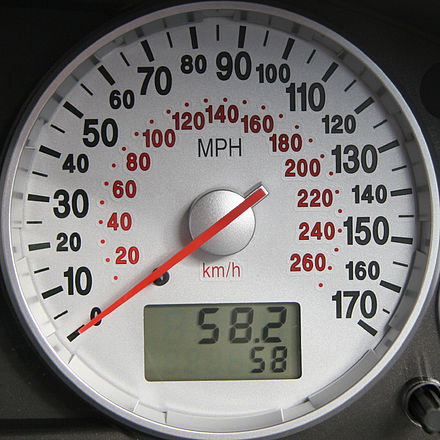
\includegraphics[width=0.5\textwidth]{speedometer}
\captionof{figure}{An old Ford speedometer.  From \href{https://commons.wikimedia.org/wiki/File:Ford_Mondeo_MK3_ST220_-_Speedometer.jpg}{Wikimedia Commons}.}
\label{fig:ch1_speedometer}
\end{center}
\begin{enumerate}
\item The Common Combinations section gives the conversion ``$1 \text{ mile/hr} =  1.609 \text{ km/hr}$''.  We can create a similar equation from the speedometer, as shown below:
\begin{equation*}
50 \frac{\text{mile}}{\text{hr}} = 80 \frac{\text{km}}{\text{hr}}
\end{equation*}
At this point, it's simple to create a similar conversion to the one given:
\begin{align*}
\frac{1}{50}50 \frac{\text{mile}}{\text{hr}} &= \frac{1}{50}80 \frac{\text{km}}{\text{hr}}\\
1 \frac{\text{mile}}{\text{hr}} &= 1.6 \frac{\text{km}}{\text{hr}}
\end{align*}

This is less than 1\% off from the more accurate value given.

\item In order to build a conversion from base units, we need our starting point (1 mph), and fix one unit at a time.
\begin{align*}
1 \frac{\text{mile}}{\text{hr}} \cdot \frac{5280 \text{ ft}}{1\text{ mile}} &= 5280 \frac{\text{ft}}{\text{hr}} \\
5280 \frac{\text{ft}}{\text{hr}} \cdot \frac{1\text{ m}}{3.281 \text{ ft}} &= 1609.3 \frac{\text{m}}{\text{hr}} \\
1609.3 \frac{\text{m}}{\text{hr}} \cdot \frac{1 \text{ km}}{1000 \text{ m}} &= 1.6093 \frac{\text{km}}{\text{hr}}
\end{align*}
We get a final result which is actually more accurate than the value given in the earlier list.
\end{enumerate}
\end{example}

Outside of an exam or quiz, it is always good to double-check unit conversions with values found online.  Typing \href{https://www.google.com/search?q=1+mph+in+kmph}{``1 mph in kmph'' into Google} pulls up a very useful unit conversion tool.

%--------------------------------------------------------------------
\section{Forms of Energy} \label{sec:ch1_energyForms}
%--------------------------------------------------------------------
The various forms of energy of interest to us are introduced in terms of a solid body having a mass m [kg]. These include potential, kinetic and internal energy.

\subsection{Potential Energy}
Potential energy (PE) is associated with the elevation of the body, and can be evaluated in terms of the work done to lift the body from one datum level to another under a constant acceleration due to gravity $g\left[\accSI\right]$, as follows:

\begin{equation}
  W=\int_{h_1}^{h_2}F\,dx=\int_{h_1}^{h_2}m\cdot g\,dx=m\cdot g(h_2-h_1)=m\cdot\Delta pe=\Delta PE
\end{equation}

Typically, we simplify this to say that $PE = mgh$.

\subsection{Kinetic Energy}
Kinetic energy (KE) of a body is associated with its velocity $V\left[\velSI\right]$ and can be evaluated in terms of the work required to change the velocity of the body, as follows:
\begin{equation}
  W=\int F\,dx=\int m\cdot a \,dx=\int m\cdot\frac{dV}{dt}dx
\end{equation}
however, velocity $V=\frac{dx}{dt}$, thus integrating from $V_1$ to $V_2$:
\begin{equation}
  W=\int_{V_1}^{V_2}m\cdot V\,dV=m\cdot\left(\frac{V_2^2-V_1^2}{2}\right)=m\cdot\Delta ke=\Delta KE
\end{equation}
Typically, this is simplified to say that $KE = \frac{1}{2} m V^2$.

\subsection{Internal Energy} \label{sec:ch1_internalEnergy}

Internal energy (U) of a body is that associated with the molecular activity of the body as indicated by its temperature T [°C], and can be evaluated in terms of the heat required to change the temperature of the body having a specific heat capacity  $c\left[\frac{\rm J}{\rm kg \cdot°C}\right]$, as follows:
\begin{equation}
  Q=m\cdot c\cdot\Delta T=m\cdot\Delta u=\Delta U
\end{equation}

Unfortunately, the specific heat $c$ changes with temperature.  For this reason, it is typically necessary to look up the internal energy of a substance from a table.

\begin{example}{Cooking with Internal Energy}

In order to gain an intuitive appreciation for the relative magnitudes of the different forms of energy we consider the (tongue-in-cheek) example of an attempt to cook a turkey by potential energy. The turkey is brought to the top of a 100 m building (about 30 stories) and then dropped from the ledge. The potential energy is thus converted into kinetic energy, and finally on impact the kinetic energy is converted into internal energy. The increase in internal energy is represented by an increase in temperature, and hopefully, if this experiment is repeated enough times the temperature increase will allow the turkey to cook. This remarkable experiment was first reported by R.C.Gimmi and Gloria J Browne – “Cooking with Potential Energy“, published in the Journal of Irreproducible Results (Vol. 33, 1987, pp 21-22).

Potential Energy
\begin{equation*}
W=\int_0^h F \ \mathrm{d}x = \int_0^h m g \ \mathrm{d}x
\end{equation*}

\begin{equation*}
\color{red}\boxed{\color{black}W=m\cdot g \cdot h=\Delta PE}
\end{equation*}

Internal Energy

\begin{equation*}
%\color{red}\boxed{\color{black}Q=m \cdot C \cdot \Delta T = \Delta U}
\redbox{Q=m \cdot C \cdot \Delta T = \Delta U}
\end{equation*}

Kinetic Energy
  \begin{align*} W &= \int F \ \mathrm{d}x = \int mg \ \mathrm{d}x = \int m \frac{\mathrm{d}{V}}{\mathrm{d}t} \ \mathrm{d}x \\ &= m \int \frac{\mathrm{d}x}{\mathrm{d}t} \ \mathrm{d}{V} = m \int_0^{{V}} {V} \ \mathrm{d}{V} \end{align*}

\begin{equation*}
  \color{red}\boxed{\color{black}W=\frac{m \cdot {V}^2}{2}=\Delta KE}
\end{equation*}

Equating all three energy forms:
\begin{equation*}
\Delta PE = \Delta KE = \Delta U \ [\rm J]
\end{equation*}

\begin{equation*}
m \cdot g \cdot h=\frac{m \cdot {V}^2}{2} = m \cdot C \cdot \Delta T
\end{equation*}

Since mass m is common, evaluate specific energy (h=100 m):
\begin{equation*}
\Delta pe = \Delta ke = \Delta u \ [\frac{\rm J}{\rm kg}]
\end{equation*}

\begin{equation*}
g \cdot h = \frac{{V}^2}{2} = C \cdot \Delta T \approx 1000 \ [\frac{\rm J}{\rm kg}]
\end{equation*}

\begin{equation*}
\frac{{V}^2}{2} \left[\frac{\rm m^2}{\rm s^2}\right] =
1000 \left[ \frac{\rm J}{\rm kg} \cdot
\left(\frac{\rm N \cdot m}{\rm J}\right) \cdot \left(\frac{1}{\rm N} \frac{\rm kg \cdot m}{\rm s^2} \right)\right]
\end{equation*}

\begin{equation*}
{V}_{\text{impact}} = \sqrt{2000} = 44.7 \left[ \frac{\rm m}{\rm s}\right] (\approx 100 \ \rm mph !)
\end{equation*}

We estimate the specific heat of a turkey.
\begin{equation*}
c = 3000 \ [{\rm J / kg ^{\circ}C}] (\text{a little less than water})
\end{equation*}

Thus
\begin{equation*}
c \Delta T = 3000 \ \Delta T = 1000 \ [{\rm J / kg}] \implies \color{red}\boxed{\color{black} \Delta T = 0.33 ^{\circ}C}
\end{equation*}

What a disappointment! At 0.33°C per fall it will require repeating the experiment 600 times just to reach the cooking temperature of 200°C.

\end{example}

%--------------------------------------------------------------------
\section{Basic Properties of Matter}
%--------------------------------------------------------------------
\subsection{Nomenclature}
\begin{tabular}{cccc}
  Symbol & Meaning & SI Units & English Units \\ \hline 
  $\rho$ & Density & $\text{kg}/\text{m}^3$ & $\text{slug}/\text{ft}^3$ OR $\text{lbm}/\text{ft}^3$ \\
  $p$ & Pressure & Pascal [Pa] & $\text{pounds}/\text{foot}$ [psf] \\
  $v$ & Specific Volume & $\text{m}^3/\text{kg}$ & $\text{ft}^3/\text{slug}$ OR $\text{ft}^3/\text{lbm}$ \\
  $T$ & Temperature & °C OR K & °F OR °R
\end{tabular}\\
\subsection{Density}
Density is the amount of mass in a given volume.  If the density is constant throughout the volume, we can say that $m = \rho \cdot {\rm Vol}$.  The units used for density are composed of a unit of mass, such as kg, and a unit of volume, such as $\rm m^3$.

The density of air under standard atmospheric conditions is around $1.2\ {\rm kg/m^3}$.  The density of water in normal conditions is about $1000\ {\rm kg/m^3}$.  Many solids have higher densities still.

\subsection{Specific Volume}
In Thermodynamics, we often prefer to use {\bf mass-specific} properties.  Mass-specific simply means that a property is given per unit mass.  Density is unfortunately volume-specific, rather than mass-specific.  In order to convert density to a mass-specific property, we simply need to invert it.  Specific volume is the result: $v = 1/\rho$, represented in $\rm m^3/kg$.

\subsection{Pressure}
Gases and liquids (together referred to as fluids) both push on all surfaces they touch.  The force they apply is based on their pressure.  If pressure is constant over the surface, we can say that $F = p\cdot A$.  A more in-depth study of this phenomenon is covered in Fluid Mechanics.

The basic unit of pressure is the Pascal [Pa], which is identical to a Newton per square meter $\left[\frac{\rm N}{\rm m^2}\right]$.  However, practical units are kilopascal [kPa], bar [100 kPa] or atm (atmosphere) [101.32 kPa]. The {\bf gauge} (or {\bf vacuum}) pressure is related to the {\bf absolute} pressure as shown in the diagram below:

\begin{figure}[H]
\centering
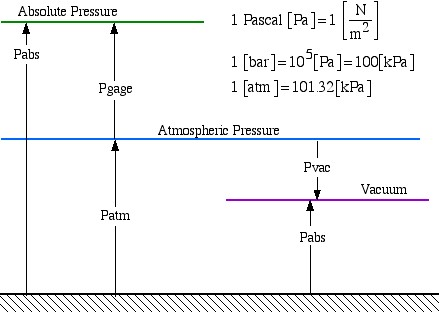
\includegraphics[width=0.75\textwidth]{Pressure}
\caption{Various pressure measurements.  Gauge and vacuum pressure are measured compared to atmosphere.}
\label{fig:ch1_pressure}
\end{figure}

The basic method of measuring pressure is by means of a {\bf manometer}, as shown below:

\begin{figure}[H]
\centering
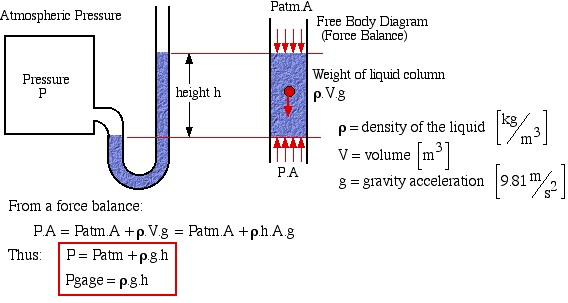
\includegraphics[width=0.75\textwidth]{Manometer}
\caption{A diagram of a manometer, which is used to find the pressure difference between two fluids.}
\label{fig:ch1_manometer}
\end{figure}

The basic principle here is that the force caused by excess pressure on one side is balanced by the extra weight of fluid on the other side.  You can find the difference in pressure through the formula $\Delta p = \rho g \Delta h$.  In this case, $\Delta p = p - p_{atm}$.

Manometers can only measure pressure differences, meaning that they are useful for gauge and vacuum pressures, but not for finding absolute or atmospheric pressure.

In order to find atmospheric pressure (and by extension, absolute pressure), a mercury {\bf barometer} can be used as follows:

\begin{figure}[H]
\centering
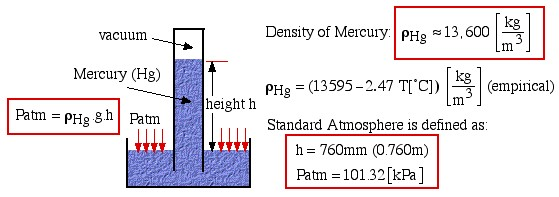
\includegraphics[width=0.75\textwidth]{Barometer}
\caption{A diagram of a barometer, which is used to find the absolute pressure of a fluid.}
\label{fig:ch1_barometer}
\end{figure}

The key here is the vacuum above the mercury.  For a pure vacuum, absolute pressure is 0.  With that knowledge, the barometer works the same as the manometer above, with $\Delta p = p_{atm} - 0$.

\subsection{Temperature}
Temperature is a measure of molecular activity, and a temperature difference between two bodies in contact (for example the immediate surroundings and the system) is the driving force leading to heat transfer between them.

Both the Fahrenheit and the Celsius scales are in common usage in the US, hence it is important to be able to convert between them. Furthermore we will find that in some cases we require the Absolute (Rankine and Kelvin) temperature scales (for example when using the Ideal Gas Equation of State).

To explain the difference between Fahrenheit and Celsius, remember that Fahrenheit describes how hot something is to a human (0 being very cold, and 100 being very hot).  Celsius does the same for water (0 being freezing, and 100 being boiling).  Rankine uses the Fahrenheit scale, but sets the zero point at absolute zero (0°R = -459.67°F).  Kelvin does the same, but for Celsius (0 K = -273.15°C).

%--------------------------------------------------------------------
\section{Types of Thermodynamic Systems}
%--------------------------------------------------------------------

For purposes of analysis we consider two types of thermodynamic systems: closed systems and open systems.

\subsection{Closed Systems}
Closed systems are usually referred to as {\bf control masses}. This type of system is separated from its surroundings by a physical boundary. Energy in the form of {\bf work} or {\bf heat} can flow across the system boundary, however there can be no mass flow across the boundary. One typical example of a system is a piston/cylinder device in which the system is defined as the fixed mass of fluid contained within the cylinder.

\begin{figure}[H]
\centering
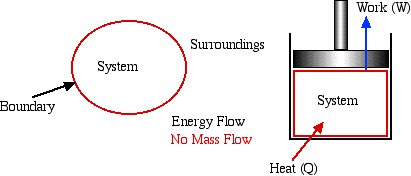
\includegraphics[width=0.5\textwidth]{ClosedSystem}
\caption{A closed system allows energy flow, but no mass flow.}
\label{fig:ch1_closedSystem}
\end{figure}

A closed system that additionally restricts energy flow is known as an {\bf isolated system}.  An isolated system will always have the same amount of mass and energy that it started with.

\subsection{Open Systems}
Open Systems are usually referred to as {\bf control volumes}. In this case, in addition to work or heat, we have mass flow of the working fluid across the system boundaries through inlet and outlet ports. In this course we will be exclusively concerned with {\bf steady flow} control volumes, in that the net mass of working fluid within the system boundaries remains constant (i.e. mass flow in = mass flow out). The following sections refer mainly to systems – we will consider control volumes in more detail starting with Chapter 4.


\begin{figure}[H]
\centering
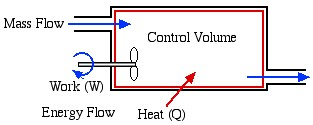
\includegraphics[width=0.5\textwidth]{OpenSystem}
\caption{An open system allows both energy flow and mass flow.}
\label{fig:ch1_openSystem}
\end{figure}

%--------------------------------------------------------------------
\section{Intensive and Extensive Properties}
%--------------------------------------------------------------------

Systems are defined by the properties of the matter that make them up.  For instance, you can define a piston by the total amount of mass inside, the temperature, the pressure, etc.  A large part of Thermodynamics is defining and calculating the properties of matter.

Properties can be either {\bf extensive} or {\bf intensive}.  Extensive properties depend on the ``extent'' of the system, meaning that if you have more mass in the system, you will have more of the property.  Key examples of this are volume and mass, though you can define any of the energies as extensive.  Intensive properties are independent of the size of the system.  Pressure and temperature are key examples, though most properties can be redefined as intensive. For instance, density ($\rho$) and specific volume ($v$) are both intensive properties defined from extensive properties.

Another example is the specific internal energy ($u$), which is simply the total internal energy ($U$) divided by mass:

\begin{equation*}
u \left[\frac{\rm kJ}{\rm kg}\right] = \frac{U\ [{\rm kJ}]}{m\ [{\rm kg}]}
\end{equation*}

In general, a {\bf specific} property is an intensive property which has been obtained by dividing the extensive property by the mass of the system.

%--------------------------------------------------------------------
\section{State and Equilibrium} \label{sec:states}
%--------------------------------------------------------------------

The {\bf state} of a system is defined by the values of the various intensive properties of the system.

The {\bf state postulate} states that if two independent intensive property values are defined, then all the other intensive property values (and thus the state of the system) are also defined. This can significantly simplify the graphical representation of a system, since only two-dimensional plots are required. Note that pressure and temperature are not necessarily independent properties, thus a boiling liquid will change its state from liquid to vapor at a constant temperature and pressure.

We assume that throughout the system {\bf equilibrium} conditions prevail, which means that there are no temperature or pressure gradients or transient effects. At any instant the entire system is under chemical and phase equilibrium, meaning that all chemical reactions and phase transitions (such as boiling) happen instantly, with no time delay.  An alternative viewpoint is that any processes (see Section \ref{sec:ch1_process}) happen slowly enough that any chemical reactions or phase transitions have a chance to complete as we inch along.

Note that this is an assumption, and that in future classes, such as Heat and Mass Transfer, you will be interested in those gradients.


%--------------------------------------------------------------------
\section{Process and Cycle} \label{sec:ch1_process}
%--------------------------------------------------------------------

A {\bf process} is a change of state of a system from an initial to a final state due to an energy interaction (work or heat) with its surroundings. For example in the following diagram the system has undergone a compression process in the piston-cylinder device.

\begin{figure}[H]
\centering
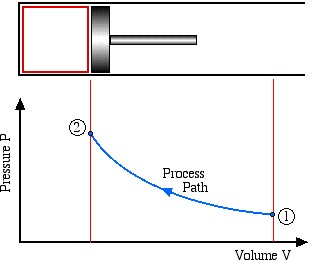
\includegraphics[width=0.5\textwidth]{BasicPistonProcess}
\caption{A compressing piston increases pressure and reduces volume in a system.}
\label{fig:ch1_process}
\end{figure}

The {\bf process path} defines the type of process undergone. Typical process paths are:
\begin{itemize}
\item Isothermal (constant temperature process)
\item Isochoric or Isometric (constant volume process)
\item Isobaric (constant pressure process)
\item Adiabatic (no heat flow to or from the system during the process)
\end{itemize}

We assume that all processes are {\bf quasi-static} in that equilibrium is attained after each incremental step of the process.

A system undergoes a {\bf cycle} when it goes through a sequence of processes that leads the system back to its original state.

% --------------------------------------------------------------------
\section{Using Software: Google Colab (Python)} \label{sec:ch1_colab}
% --------------------------------------------------------------------
\href{https://colab.research.google.com}{Google Colab} is a free IDE (integrated development environment) for Python.  Through Colab, you can write Python code, link to countless existing libraries of code and data, and run the code you write.

\subsection{Setup and CoolProp Basics}
To start off, click the link above (or search Google for ``Google Colab'').  You want to create a New Notebook, so either select the option from the pop-up menu, or select ``File'' from the menu bar and click on ``New notebook''.

Your empty notebook should look something like Figure \ref{fig:ColabScreenshot1}.

\begin{figure}[H]
\centering
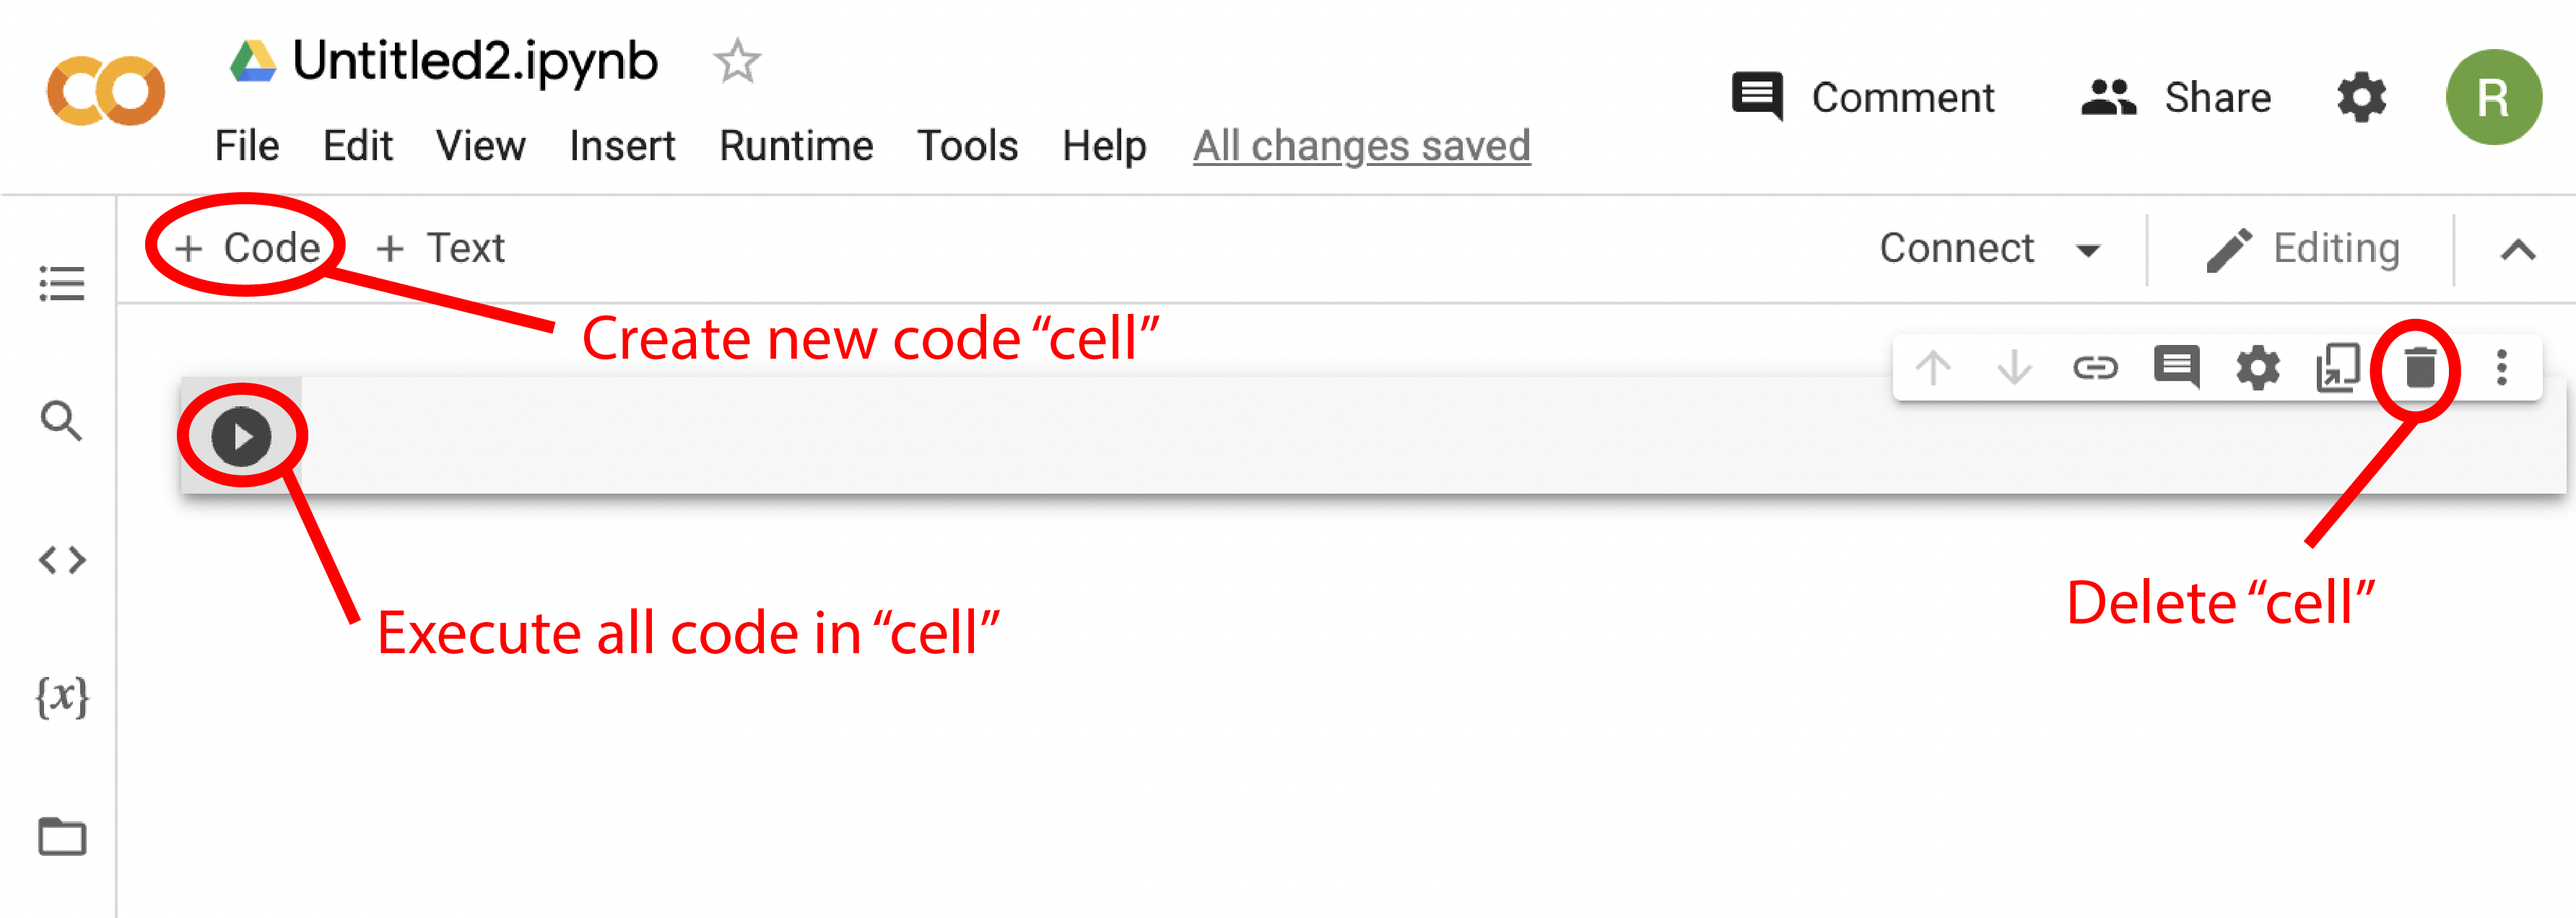
\includegraphics[width=0.9\textwidth]{ColabScreenshot1_labelled}
\caption{An empty notebook in Google Colab, with several important buttons labeled.}
\label{fig:ColabScreenshot1}
\end{figure}

Once you have your notebook created, we need to start off with some commands to link to some common libraries:

\begin{Verbatim}[commandchars=\\\{\}]
\textcolor{OliveGreen}{# Clear all variable definitions}
\textcolor{blue}{\%reset} -f                         
\textcolor{violet}{from} numpy \textcolor{violet}{import} *               \textcolor{OliveGreen}{# Import common numerical functions (like sqrt)}
\textcolor{violet}{from} matplotlib.pyplot \textcolor{violet}{import} *   \textcolor{OliveGreen}{# Import plotting functions (like plot)}
\end{Verbatim}

Everything to the right of the \# symbol is a comment (text that is ignored by Python).  Comments are not part of the code, but are helpful in describing the code in plain language.

The \texttt{reset} command removes variable definitions, and essentially makes sure we're working from a clean slate.  Some of the most frustrating errors to debug stem from the fact that something is defined in a way that you aren't expecting, and this helps avoid some of those errors.

The \texttt{from ... import *} command grabs all of the functions from a library and gives us access to them.  We are getting function from the \texttt{numpy} library and the \texttt{matplotlib} library.  The \texttt{numpy} library contains functions like \texttt{sqrt}, \texttt{sin}, and \texttt{log}, and generally allows you to do everything you could do on a scientific calculator (plus a lot more we won't talk about here).  The \texttt{matplotlib} library gives you access to \texttt{plot} and all the functions you need to make plots look good.

\subsection{Basic Math} \label{sec:pythonBasics}

Let's say that we know the area of a square (in acres) and would like to find out the length of one of the sides.  We can make this happen through the following lines of code:

\begin{Verbatim}[commandchars=\\\{\}]
areaInAcres = \textcolor{JungleGreen}{2.5}  \textcolor{OliveGreen}{# 2.5 acres}
areaInSqFt = areaInAcres*\textcolor{JungleGreen}{43560}  \textcolor{OliveGreen}{# conversion to square feet}
sideLength = sqrt(areaInSqFt)   \textcolor{OliveGreen}{# Area = length^2}
\end{Verbatim}

This will convert from acres to square feet, then take the square root in order to find the length of one of the sides.  Running this code will not produce any errors, but at the same time, it won't seem to do anything.

In order to get information out of the code, we need to use the \texttt{print} command.  The simplest form is shown below:
\begin{Verbatim}[commandchars=\\\{\}]
print(sideLength)
\end{Verbatim}
This will output the numerical value of \texttt{sideLength}, but nothing else.  The problem with this arises when you are printing several different values over the course of your code.  It becomes very easy to forget which number is which, or at the very least waste time trying to figure it out.

What I prefer is a slightly more complicated version that includes a label and units:
\begin{Verbatim}[commandchars=\\\{\}]
print(\textcolor{purple}{'length = '}, sideLength, \textcolor{purple}{'m'})   
\end{Verbatim}

The little bit of up-front effort means that you are less likely to forget what the number means in the future.

\subsection{Plotting in Python}

In order to make a plot, we first need to accumulate some data.  The easiest way of doing this is to manually build a {\bf list}.  Once you have two lists, you can plot!  You can do this with the following three lines of code:
\begin{Verbatim}[commandchars=\\\{\}]
X = [0, 1, 2, 3, 4]
Y = [4, 1, 0, 1, 4]
plot(X,Y)
\end{Verbatim}

After running, you should end up with a screen that looks like Figure \ref{fig:ColabScreenshot2}

\begin{figure}[H]
\centering
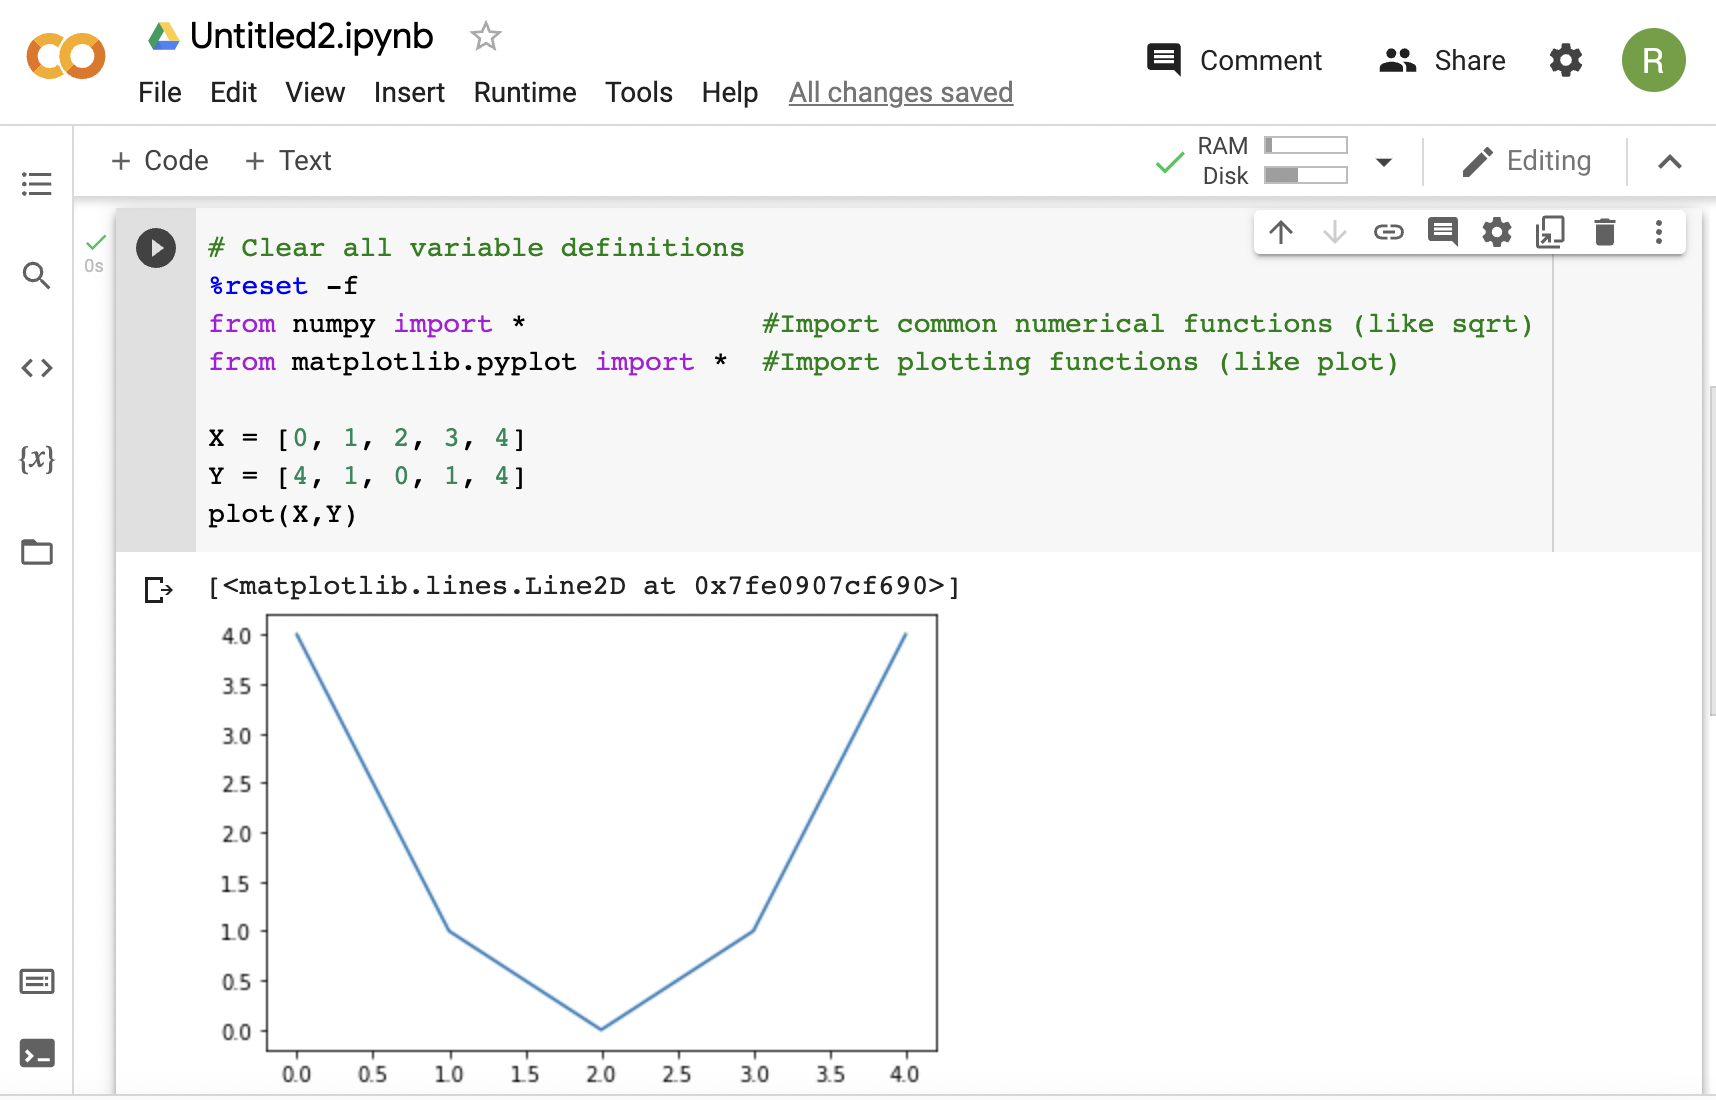
\includegraphics[width=0.9\textwidth]{ColabScreenshot2}
\caption{Google Colab, displaying a simple plot.}
\label{fig:ColabScreenshot2}
\end{figure}

We could give labels, titles, etc., but there's not much point when our data doesn't actually mean anything.  Instead, let's return to our original problem of find the side length of a plot of land.

In order to attack this problem, we will build a list and calculate our side length values all at once.  To start, we need to define all of the areas we want to work with.  Instead of manually putting those in a list, we will use the \texttt{linspace} command:

\begin{Verbatim}[commandchars=\\\{\}]
areaInAcres = linspace(0, 25, 100) \textcolor{OliveGreen}{# create 100 points between 0 and 25}
\end{Verbatim}
\texttt{linspace} has three {\bf arguments}, or input values.  The first and second define the beginning and ending points of the list, respectively.  The last argument is the number of points.  If you want to see all the values in the list, you can use the command \texttt{print(areaInAcres)}.

Python can actually work with lists for most simple functions (like multiplication, \texttt{sqrt}, trig functions, etc.).  This means we can re-use the code we wrote for Section \ref{sec:pythonBasics}:

\begin{Verbatim}[commandchars=\\\{\}]
areaInAcres = linspace(0, 25, 100) \textcolor{JungleGreen}{2.5}  \textcolor{OliveGreen}{# 2.5 acres}
areaInSqFt = areaInAcres*\textcolor{JungleGreen}{43560}  \textcolor{OliveGreen}{  # conversion to square feet}
sideLength = sqrt(areaInSqFt)   \textcolor{OliveGreen}{  # Area = length^2}
\end{Verbatim}

Then, we can plot \texttt{areaInAcres} as the x-axis, and \texttt{sideLength} as the y-axis.

\begin{Verbatim}[commandchars=\\\{\}]
plot(areaInAcres, sideLength)
\end{Verbatim}

This will give us a plot, but since our line actually has meaning, we should give the plot labels and a title.  While we're at it, we'll also modify the axes and add grid lines.

The label and title commands are very straightforward.  The important thing to note is that the arguments must be {\bf strings}, which are collections of characters.  You denote a string using quotation marks.

\begin{Verbatim}[commandchars=\\\{\}]
xlabel(\textcolor{purple}{'Plot Area [ac]'})
ylabel(\textcolor{purple}{'Side Length [m]'})
title(\textcolor{purple}{'Length of Side of Land vs. Acreage'})
\end{Verbatim}

Next, we'll use the \texttt{axis} command.  \texttt{axis} takes a list of values as an argument, which should be in the order \texttt{[<xmin>, <xmax>, <ymin>, <ymax>]}.  We'll implement this as follows:
\begin{Verbatim}[commandchars=\\\{\}]
axis([0, 25, 0, 1200])
\end{Verbatim}

Finally, let's add some grid lines to make data a little easier to extract.
\begin{Verbatim}[commandchars=\\\{\}]
grid(visible=True)
\end{Verbatim}

When you've put everything together, Colab should look like Figure \ref{fig:ColabScreenshot3}.

\begin{figure}[H]
\centering
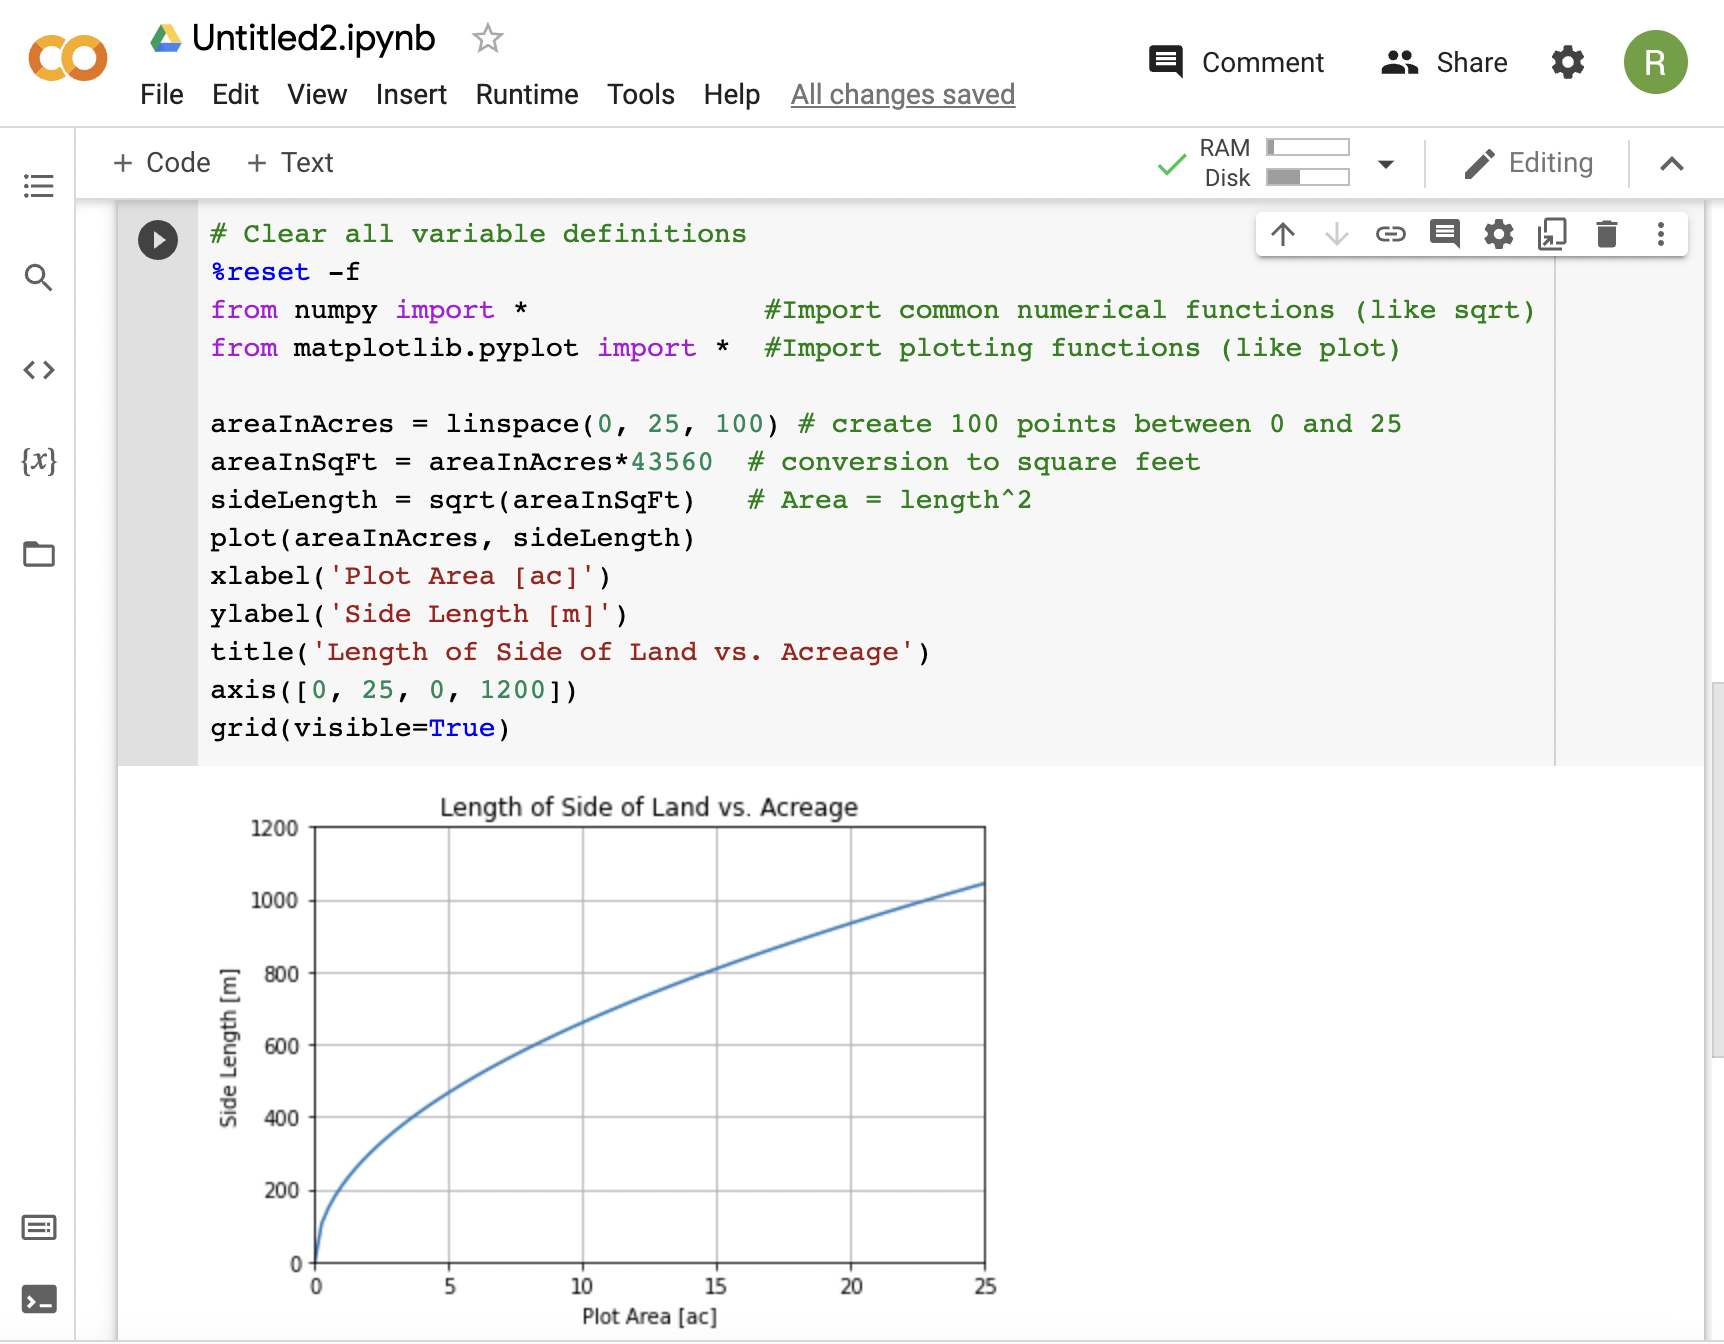
\includegraphics[width=0.9\textwidth]{ColabScreenshot3}
\caption{Google Colab, displaying a fully labeled plot.}
\label{fig:ColabScreenshot3}
\end{figure}

\begin{homework}
%--------------------------------------------------------------------
\question How are states, processes, and cycles related?
%--------------------------------------------------------------------
\question Describe the difference between an intensive and extensive property.
%--------------------------------------------------------------------
\question For each of the following properties, state whether it is intrinsic or extrinsic.
\begin{itemize}
\item Pressure
\item Volume
\item Kinetic energy
\item Specific internal energy
\end{itemize}
%--------------------------------------------------------------------
\question For each of the following systems, state whether it is open, closed, and/or isolated.
\begin{itemize}
\item The ice and water inside of a well-insulated cooler
\item An airtight piston, which is heated from the outside
\item A water spigot
\end{itemize}
%--------------------------------------------------------------------
\question Describe the difference between an isothermal process and an adiabatic process.

%--------------------------------------------------------------------
\question A soda can has a diameter of 2.13 inches and a height of 4.83 inches.  Additionally, it has a mass of 384 g.  Assuming the can is perfectly cylindrical, and the mass of aluminum is 14.7 g, determine:
\begin{itemize}
\item The volume of soda in the can (in ${\rm ft^3}$). \answer{[0.0100 ${\rm ft^3}$]}
\item The mass of soda in the can (in lbm). \answer{[0.812 lbm]}
\item The density of soda in the can (in $\frac{\rm kg}{\rm m^3}$) \answer{[1304 $\frac{\rm kg}{\rm m^3}$]}
\end{itemize}
%--------------------------------------------------------------------
\question The temperature in Chicago in winter can be as low as 14°F. What is the temperature in °C, K, and °R?
%--------------------------------------------------------------------
\question A piston with a diameter of 3'' compresses air, which is at an {\bf absolute} pressure of 2 atm.  What is the net force required to hold the piston still? Provide your answer in lbf. \answer{[103.9 lbf]}


Hint: don't forget atmosphere ($p_{atm}=1 \rm\ atm$) pushing on the other side.
%--------------------------------------------------------------------
\question Rework the previous question in Google Colab.  Plot the force required to hold the piston still, while varying the diameter of the piston between 1'' and 10''.  Plot your result, including a title and labels on both the x- and y- axes.
%--------------------------------------------------------------------
\question A barometer measures 690 mmHg.  What is the atmospheric pressure in kPa? \answer{[92 kPa]}
%--------------------------------------------------------------------
\question A manometer connects a tank with an unknown pressure to atmosphere.  If the manometer is filled with water at 20°C ($\rho = 1000 {\rm kg/m^3}$), and a height difference of 20 cm is measured, what is the gauge pressure in Pa?  \answer{[1962 Pa]}  If the atmospheric pressure is 101 kPa, what is the absolute pressure in Pa? \answer{[102.96 kPa]}
%--------------------------------------------------------------------
\end{homework}

